
\chapter{Detecting and injecting binaries}
\label{Chap:BinAlgo}

In this chapter, we introduce a new algorithm to detect and record binary system in N-body simulations, then calibrate its free parameter. With this tool, we analyse the spontaneous binary population arising in the \HubLem systems and we describe a binary injection method to complete this population to match the observations.


\minitoc

\section{A new binary detection algorithm}


\subsection{Density comparison}

The study of binary populations in N-body simulations requires an algorithm to detect binary systems and compute their characteristics. The simplest approach is to compute all star-star energies and consider bound pairs as binaries. This records a lot of ephemeral interactions, as N-body dynamics cause transient bound systems. An additional criteria is needed to assess the stability and robustness of a pair as a binary.

\begin{figure}
\begin{center}
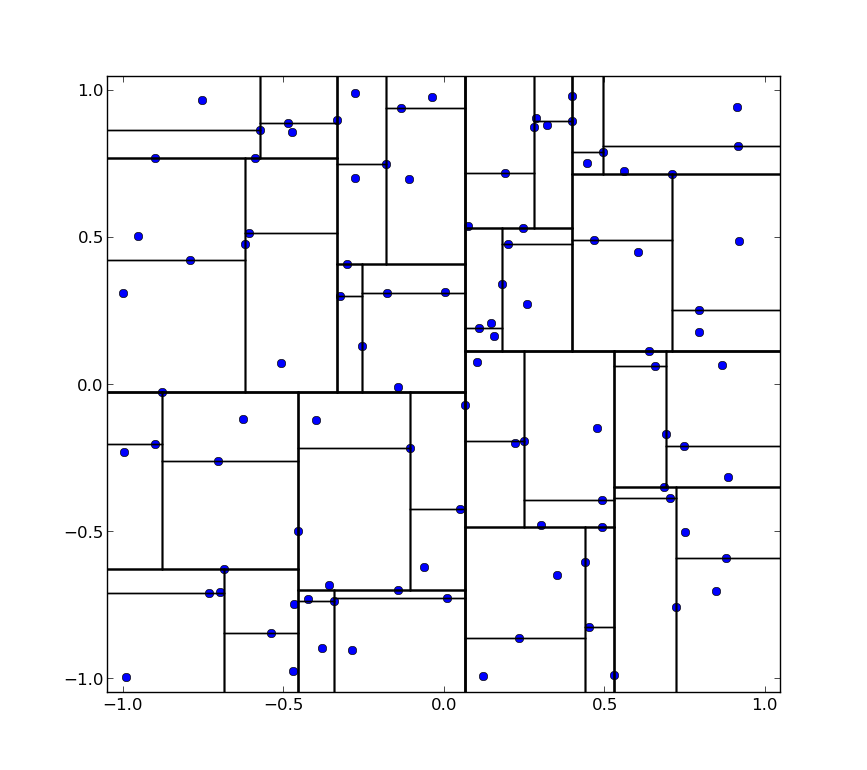
\includegraphics[width=0.6\textwidth]{Figures/5_kdtree}
\caption{Illustration of a KD-tree for a random two-dimensional distribution (blue dots).}
\label{Fig:5_kdtree}
\end{center}
\end{figure}


We introduce a new algorithm based on the idea of a density threshold: binaries must be denser than their direct environment. Before describing the algorithm, we wish to emphasize the importance of neighbour searches in this kind of study. Be it to obtain bound pairs or to study said pair direct environment, the quick retrieval of neighbours is crucial to an effective algorithm.

The method described here relies on the KD-tree algorithm \citep{numericalrecipes}. While brute-force neighbour searches scale as $\propto N$, as all stars in the system have to be checked as potential neighbours, a KD tree, once built, performs neighbour searches with algorithmic complexity $\propto\log (N)$. The tree is built by sorting particles along one dimension, splitting them at the median, then sorting each branch along another dimension, splitting them again, and so on, cycling over dimensions. A two-dimensionnal example is show on Fig~\ref{Fig:5_kdtree}.





First, binary candidates are identified as negative energy pairs. The semi-major axis of the system is derived from the star motions, then a "binary density" is computed, with $a$ the binary's semi-major axis :
\begin{equation}
 \rho_{binary} = \frac{m_1 + m_2 }{4\pi a^3/3 }\, .
\end{equation}
This is then compared to the local neighbour density, defined as the cumulated mass of a fixed number $N_{nb}$ of neighbours to the pair over the spherical volume reaching to the last neighbour.
\begin{equation}
 \rho_{local} =  \frac{\sum\limits_{i=0}^{N_{nb}} m_i}{ 4 \pi r_{N_{nb}}^3 /3} .
\end{equation}


\begin{figure}
\begin{center}
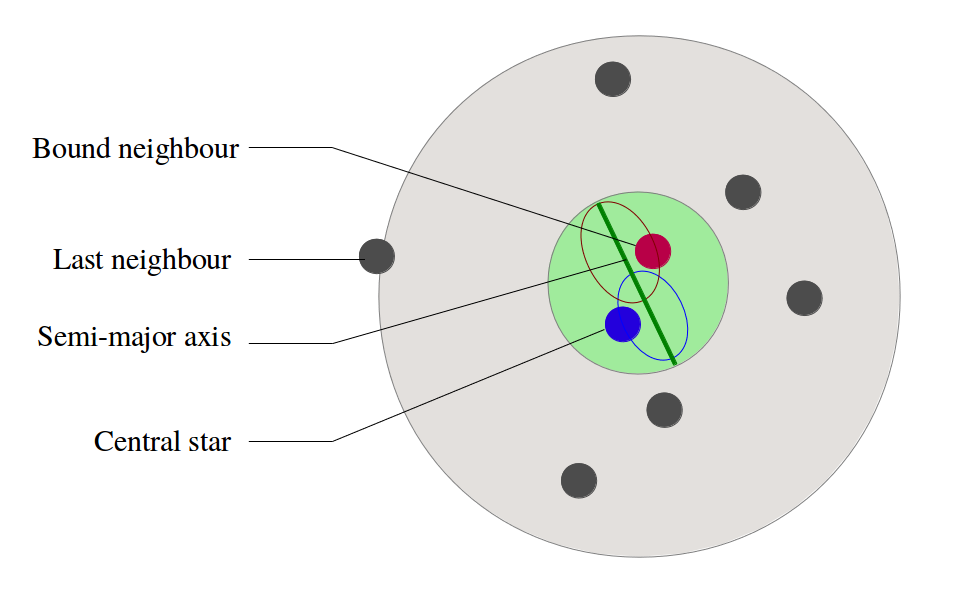
\includegraphics[width=0.6\textwidth]{Figures/5_neighbours}
\caption{Illustration of the density threshold method. The central blue stars and the red bound neighbour describe a two-body orbit shown on the figure while the green bar indicates the major-axis of the system. This defines the binary density over the green sphere, while the local density is defined with the grey stars, the other neighbours. $N_{nb}$ was here set to 7. }
\label{Fig:5_neighbours}
\end{center}
\end{figure}




If the density ratio exceeds a threshold $D$, 
\begin{equation}
\label{Eq:density_ratio}
\frac{ \rho_{binary} }{ \rho_{local} } > D,
\end{equation}
the pair is registered as a binary.  Other authors, eg \cite{Parker2009,Lomax2015}, have used close hybrids of the criteria that we have implemented.

Stars can be found to be part of several binaries at once, which happens more often for massive stars as they clear more easily the density threshold. When that happens, the algorithm selects from such connected systems only the pairs exhibiting the lowest (most negative) binding energy.

This method has two free parameters: $N_{nb}$ and $D$. $N_{nb}$ can be set from 6 to 10 neighbours without a substantial impact on the detection. The density ratio is a more critical parameter, as if it is chosen too low, a lot of ephemeral binaries are found, while a high value picks only the closest binaries, ignoring wider, yet stable, systems.



\subsection{Choosing a density ratio}



\begin{figure}
\begin{center}
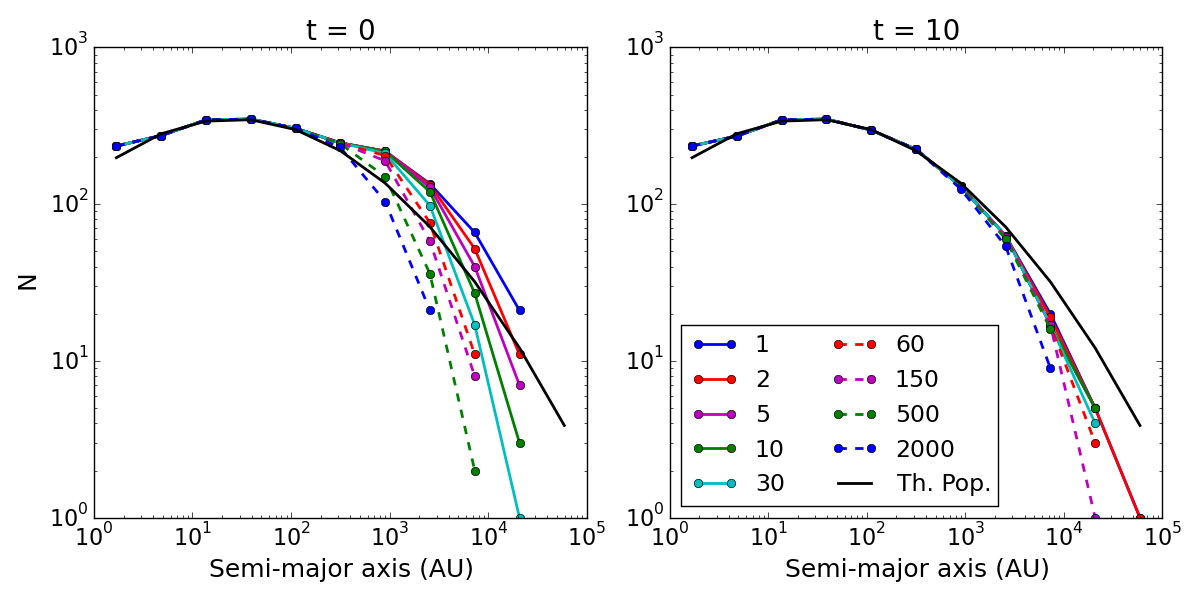
\includegraphics[width=\textwidth]{Figures/5_sm_ratios}
\caption{Semi-major axis histograms for various value of the density ratio $D$ at t=0 and 10 H.u for a N = 10k King model and a binary fraction $f_b =0.3$. The injected log-normal population is shown as a black solid line.}
\label{Fig:5_sm_ratios}
\end{center}
\end{figure}



We wish to find a good compromise value for the critical density ratio $D$ that maximizes the number of detected stable binaries without collecting too much transient system. To do so, we explore the results brought by different values of $D$ in a N-body system containing binaries.

We create a virialized King model with N = 10000 stars and a binary fraction of 0.3. This means there are 2300 binaries and 5400 single stars,
\begin{equation}
f_b = \frac{N_b}{N_s + N_b} = \frac{N_b}{N-N_b} \quad \implies \quad N_b = \frac{f_b}{1+f_b} N = 2300.
\end{equation}

The binaries follow the \cite{Raghavan2010} log-normal distribution introduced in \ref{Sec:0_raghavan}. We let the system run for 10 H.u, or 12 crossing times, and write a snapshot every 0.1 H.u.

The binary detection is ran over all snapshots once per density ratio in the following list:

\begin{center}
\begin{tabular}{l|rrrrrrrrr}
\centering
D  &  2000 & 500 & 150 & 60 & 30 & 10 & 5 & 2 & 1\\ 
\end{tabular}
\end{center}

We show on Fig~\ref{Fig:5_sm_ratios} the semi-major axis distribution retrieved for various $D$ for t=0 and t=10, with the theoretical injected population as a solid black line.



\begin{figure}
\begin{center}
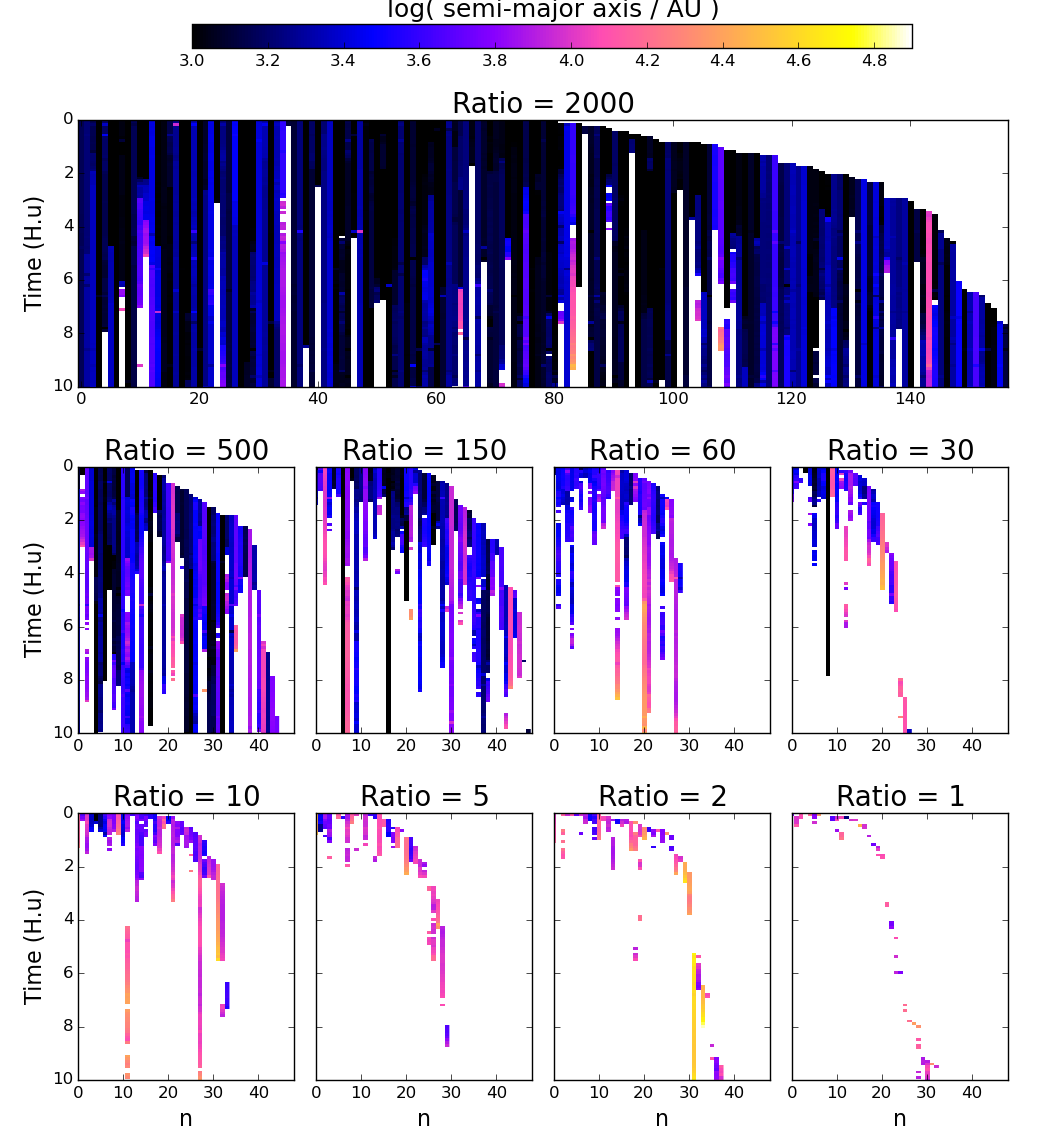
\includegraphics[width=0.9\textwidth]{Figures/5_flickering}
\caption{Visualization of the wide ($a>1000$ AU) binary population in a King model over time. Large upper panel show the evolution of all binaries detected for a density ratio $D=2000$, ordered by time of first detection. Each lower sub-panel show the new binaries detected with the new, lower, value of $D$ compared to the previous one.}
\label{Fig:5_flickering}
\end{center}
\end{figure}

Looking at the left panel, for t=0, we see all density ratios return the same population for $a < 1000$ AU, while for higher separation, there are large variations. $D = 2000$ does not detect semi-major axis larger than 3000 AU, while $D = 1$ detects $\sim$ 30 systems with $a > 10^4$ AU. After 12 crossing times, on the right panel, we can see the detected tight population did not change, while all wide populations converged. The population detected with the highest ratios did not significantely evolve, while low ratios saw a large depletion of the population they initially returned. 

 We can say that a very high ratio only detect binaries that are garanteed to resist the dynamical processing and survive, while low ratios detect more fragile systems. How ephemeral are these latter binaries ? To evaluate the different population detected by different ratios, we show on Fig~\ref{Fig:5_flickering} the detailed evolution of the wide, $a>1000$ AU population. The large upper panel show all wide binaries evolution (time on y-axis) for $D=2000$, arranged on the x-axis by time of first detection. Each pixel column represents a binary. The smaller sub panels show, for each density ratio, the history of the binaries this ratio detected that the previous, greater ratio did not. A binary that is detected with $D=2000$ will also be detected for $D=500$ and any other lower value. Fig~\ref{Fig:5_flickering} shows what kind of binaries lowering the ratio progressively brings in the detected population. The color codes the logarithm of the semi-major axis in AU, white means the binary is not detected.

The $D=2000$ population is mainly made of stable, relatively tight binaries. About half the binaries are detected at t=0, while the others dynamically form in the system. Some are destroyed, other widened through interactions as their color bars transitions to a lighter color, sometimes after a ``flickering" phase, when the detection goes on and off over successive snapshots. This is due to the binary entering a dynamical interaction with a third star or other binary, making the neighbour density undergoing spikes. This interaction leaves the binary with a weaker bound, thus larger separation. 

Looking at the populations brought by lower ratios, we see they are progressively wider and more transient/flickering as the ratio lowers, which is to be expected. $D=1$ only brings very ephemeral pairs, often not lasting more than a single snapshot. All ratios bring their share of transient binaries, but $D=10$ is the last to capture relevant, relatively long-lived pairs.

Extreme values of density ratios bring a large difference in the detection of large binaries, but a moderate value like $D=10$ appears the best compromise to capture the substance of a binary population.










\section{The spontaneous binary population} 
\label{Sec:5_spontaneous}



Star-star interactions which take place during the HL expansion phase speed up the internal evolution of small substructures (or, clumps). The global expansion, on the other hand, brings about correlations in phase-space coordinates and the formation of loose binary stars (see Appendix~\ref{App:phasespace} and \citealt{Kouwenhoven2010,Moeckel2011}). We refer to that population of binary stars as {\it spontaneous} binaries in the following. There is a trade off between the creation of spontaneous binaries, and their destruction / heating when they sit near or inside a clump. We address statistically their properties as a sub-population through numerical experiments.

We set up 20 models with N=20k stars drawn from the $L_3$ single star initial mass function (IMF) of \cite{Maschberger2013}. The $L_3$ IMF  matches the better known \cite{Kroupa2001a} and \cite{Chabrier2003} functional forms but with fewer free parameters. We set a lower truncation mass of 0.1~$\Mo$ and a maximum of 30~$\Mo$, for an average mass of 0.5~$\Mo$. This choice of truncation values allows us to take into account the impact of massive stars on the dynamics, while keeping the vast majority of stars on the main sequence for up to 18 Myr, which is the maximum simulation run-time in next chapter. For now we only look at the fragmented models without considering for the further dynamical evolution.


\subsection{Binary fraction vs primary mass}
\label{Sub:spontaneous_binaryfractions}

Several studies have found a strong correlation between the binary fraction $f_m$ and the primary mass $m$ of a binary system (for compilations, see e.g. Fig. 17 of \citealt{Bate2012} and Fig. 12 of \citealt{Raghavan2010}). Since heavy stars tend to drive the formation of clumps in HL models, by attracting stars to themselves, it is natural to expect the HL procedure to give rise to a correlation of that nature.  



\begin{figure}
\begin{center}
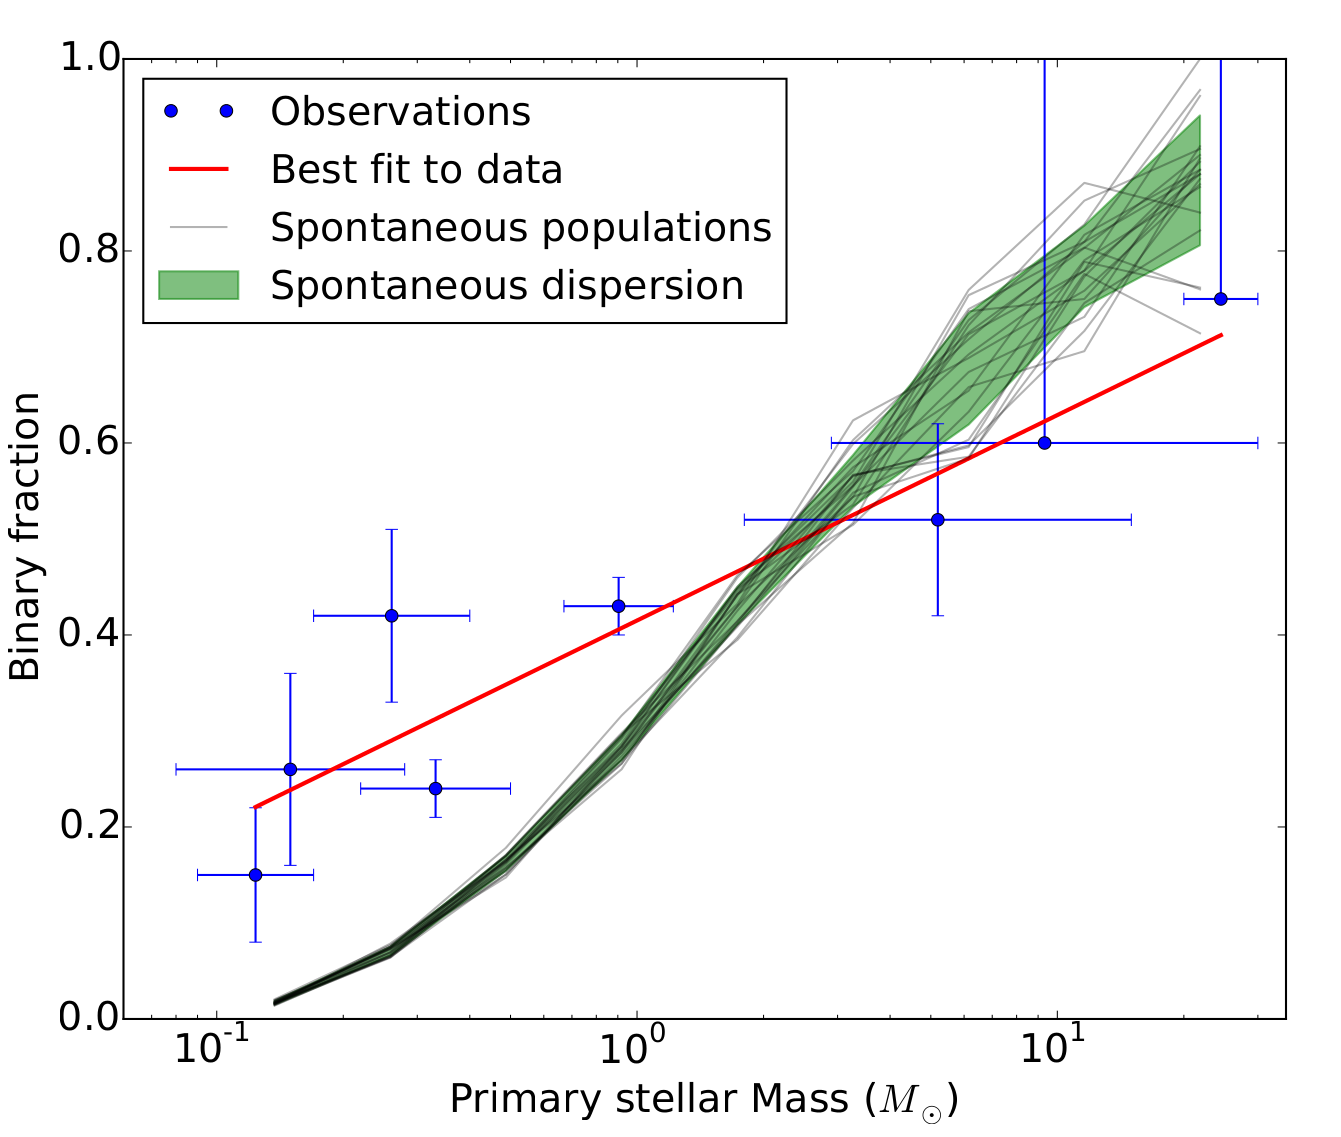
\includegraphics[width=0.7\textwidth]{Figures/5_spontaneous_primarymass}
\caption{Observational data of binary fractions (dots with uncertainties) as a function of primary mass. The data are taken from (in increasing primary mass): \protect\cite{Close2003,Basri2006,Fischer1992,Ward-Duong2015,Raghavan2010,Patience2002,Preibisch1999,Mason1998}. The red line is a  best-fit linear relation. The thin curves and 1-$\sigma$ dispersion shaded area are the results for a population of  spontaneous binaries obtained from HL  models.}
\label{Fig:5_spontaneous_primarymass}
\end{center}
\end{figure}




The spontaneous binary fractions found in our 20 \HubLem models for logarithmic primary mass bins are plotted as black lines on Fig~\ref{Fig:5_spontaneous_primarymass}. The shaded area shows the 1-$\sigma$ dispersion for these distributions. The fraction increases rapidly  with primary mass,  and is in close agreement with the data for primaries of mass higher than 2 $M_\odot$, when $f_m$ exceeds 50\%.  However, the HL  models show  a significant deficit of low-mass primary binaries in comparison to observational data.  

The high binary fraction for heavy primaries can be explained, at least in part,  by considering the mass segregation occurring in the clumps during their formation. We shown in Chapter \ref{Chap:nbody} that massive stars tend to sink to the center of clumps. These high mass stars are more likely to capture another star to form a binary through a three-body interaction as they sit in denser environments \citep{Spitzer1987}. A heavy star also creates a deeper potential well wherein to trap a fly-by star at the on-set of HL fragmentation. There is indirect evidence for the three-body binary formation process to draw from mass-segregated clumps, because these binaries have a mean mass ratio $q = m_2/m_1$  that is significantly \textit{larger} than expected from random pairing. The mean value of $q$ for  binaries with a primary star in the range $15-30 M_\odot$  is $0.21 \pm 0.11$, whereas random pairing  yields a mass ratio of $0.02 \pm 0.02$ for that mass range. Due to mass segregation inside clumps, massive stars are more likely to pair up with moderately heavy companions rather than light ones.



\subsection{Spontaneous semi-major axis distribution}
\label{Sub:spontaneous_separations}

The distributions of semi-major axes $a$ and orbital  periods are the main parameters used to 
characterise binary populations. Up to this point, the distances were given in  computational N-body units. To convert the models to physical scales, we matched their stellar number density within the half-mass radius to those of observed clusters.  \cite{King2012a}  compiled  data for several young clusters and gave their stellar densities within half-mass radii, with high values reaching  400 stars$/pc^3$, typical of the ONC, and low-densities  of $\sim 6$ stars$/pc^3$, more akin to the Taurus region. These are the two reference values used to build up our dataset of numerical models. The time conversion gives a physical free-fall time of the models of 0.76 Myr for the high density clusters and 6.0 Myr for the low density ones.



\begin{figure}
\begin{center}
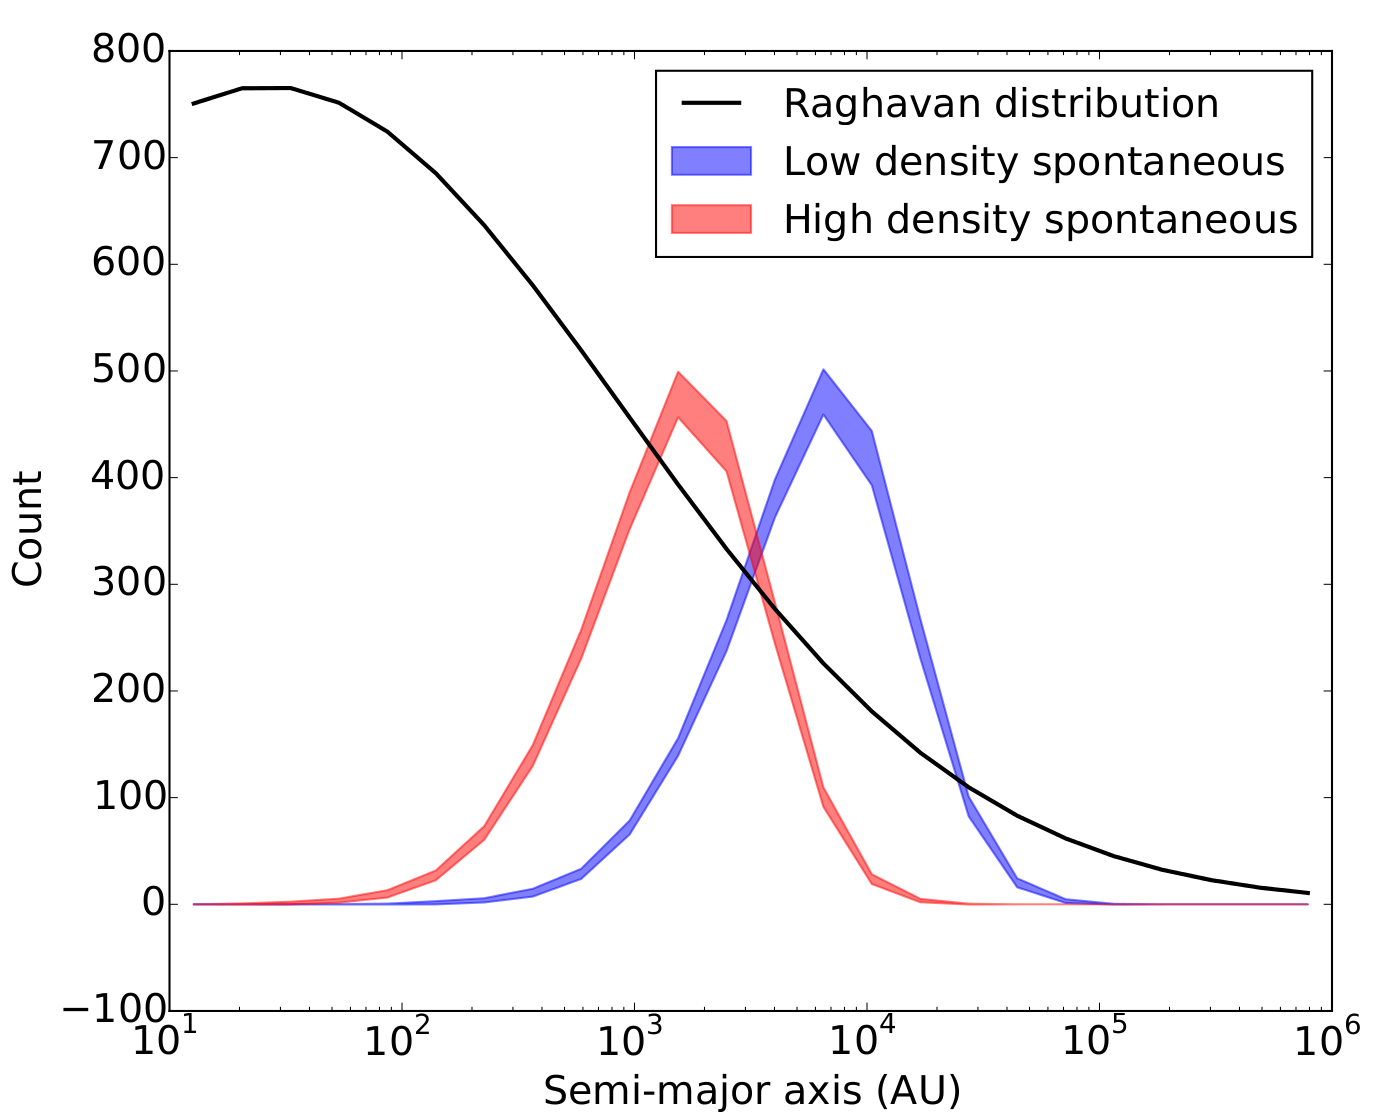
\includegraphics[width=0.7\textwidth]{Figures/5_spontaneous_smaxis}
\caption{Distribution of semi-majors axes of spontaneous binary populations for two values of stellar number density. Green curve show the canonic separation distribution from \protect\cite{Raghavan2010}. }
\label{Fig:5_spontaneous_smaxis}
\end{center}
\end{figure}


In practice the spontaneous binaries develop a bell-shaped  distribution of separation centered on $\sim 2000$ AU for a high-density HL model,  and $\sim 7000$ AU for a low-density one, shown on Fig.~\ref{Fig:5_spontaneous_smaxis} for the same 20 models than before. The spread shows the 1-$\sigma$ dispersion. This is much wider than the averaged value of $\sim 50$ AU for the Galactic field population \citep{DM91,Raghavan2010}, where separations of $\sim 1 $ AU or lower are not uncommon. Hydrodynamical calculations by \cite{Bate2012} show that orbital energy dissipated in the early stages of formation may cause binaries with $ a \sim 10 $ AU  separation to shrink to $ a \sim  0.5 $ AU in the course of $t \sim 1 $ Myr. Analytical arguments by \cite{Stahler2010} and \cite{Korntreff2012} would have external drag forces from residual gas drive a tight binary to merge completely. \cite{Kroupa2001} have shown that stellar collisions  alone can not bring a narrow distribution of semi-major axes to the full width of observed values. Other authors such as \cite{Parker2014} investigated the evolution of a binary population identical to the field but embedded in clumpy, fractal clusters \citep{Goodwin2004} to test the robustness of the field population. 
A full spectrum of separations is desirable for comparison with data and theoretical models but is not a  natural outcome of the HL fragmentation. 

We follow \cite{Parker2014} to ease comparison with their setup, by supplementing the population of spontaneous binaries with one that matches the field galactic populations at small $a$. 
In doing so, we should also constrain the primary mass distribution so as to redress the deficit of small-mass primaries (Fig.~\ref{Fig:5_spontaneous_primarymass}).



\subsection{Completing the population}
\label{Sec:Completing}

\subsubsection*{Completion procedure}


\begin{figure}
\begin{center}
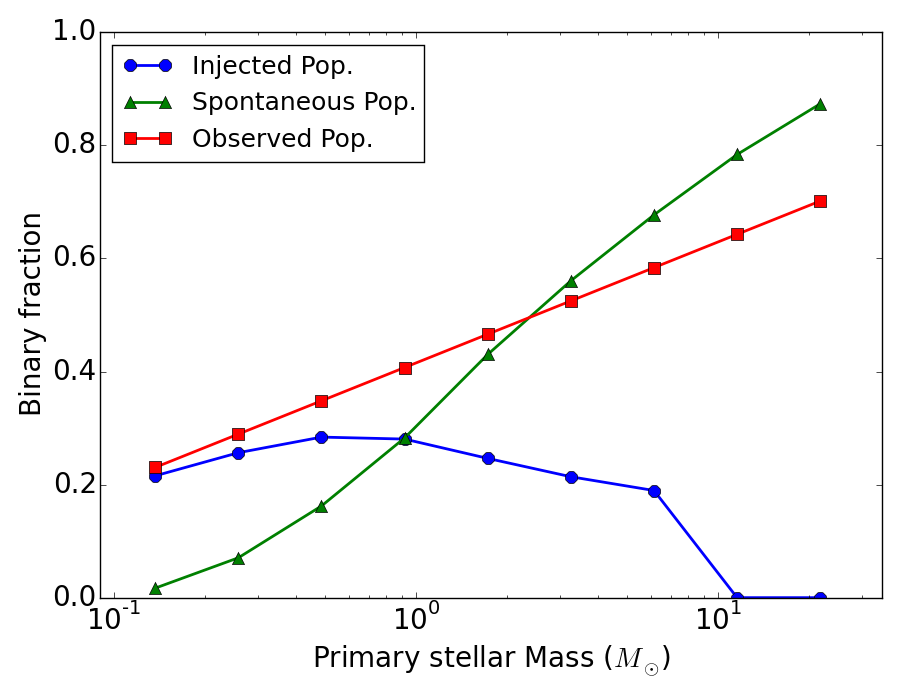
\includegraphics[width=0.7\textwidth]{Figures/5_injected_fraction}
\caption{Binary fraction as a function of primary mass. Blue circles show the binary fractions in the population injected to complete the spontaneous binaries, in green triangles. The target, observed, fractions are showed as red squares. }
\label{Fig:5_injected}
\end{center}
\end{figure}

The addition of new binaries to the HL distribution is not straightforward, as the phase space coordinates of stars in an HL fragmented system are the consequence of the numerical evolution during the expansion (no known functional distribution function). A practical and coherent method is to build the extra binary population \textit{before} the HL expansion phase, and split them at apex.

The first step is to choose the proper distribution of primary mass for these new binaries. It should take into account the spontaneous population to preferentially populate the low-mass primary space. It should also take into account the fact that as the system expands with an effective number of stars $\tilde{N} = N - n_{in}$ with $n_{in}$ the number of injected binaries, as these contain two stars fused in a single object until apex. Thus, the number of spontaneous binaries is reduced. Moreover, some spontaneous pairs form at the end of the HL phase with one fused binary as a component. Many of these spontaneous binaries (we found $\approx 50\%$)  are no longer classified as bound pairs  once the point mass component is split into the binary. 

By making a few assumptions, it is possible to account for these influences and derive a distribution of primary masses consistent with a final binary fraction distribution close to observations. The procedure is detailed in appendix \ref{App:completion}. Once primaries are picked, secondaries are chosen through random pairing in the remaining population and fused binaries are introduced in the uniform, pre-expansion model. The injected population is shown as the blue curve on Fig~\ref{Fig:5_injected}. Binaries are still injected at moderately high masses, even though the spontaneous population had enough binaries in this range, because some of these binaries will not survive when their secondary component splits. They have to be replenished.



Once the expansion ends and before binary splitting, the semi-major axis distribution of spontaneous binaries is measured. A semi-major axis completion distribution is obtained by subtracting the semi-major axis distribution from spontaneous (only considering the ones expected to survive) from the \cite{Raghavan2010} distribution, so the final population recovers the observed population as much as possible. The injected binaries are split with semi-major axes drawn from this completion distribution. 

%The binary detection algorithm is then ran on the system, bringing the resulting population. Binary fraction as a function of primary mass is seen on Fig~\ref{Fig:5_completed_primarymass}, while the semi-major axis distribution is shown as the green curve on Fig.~\ref{Fig:5_completed_smaxis}.



\begin{figure}
\begin{center}
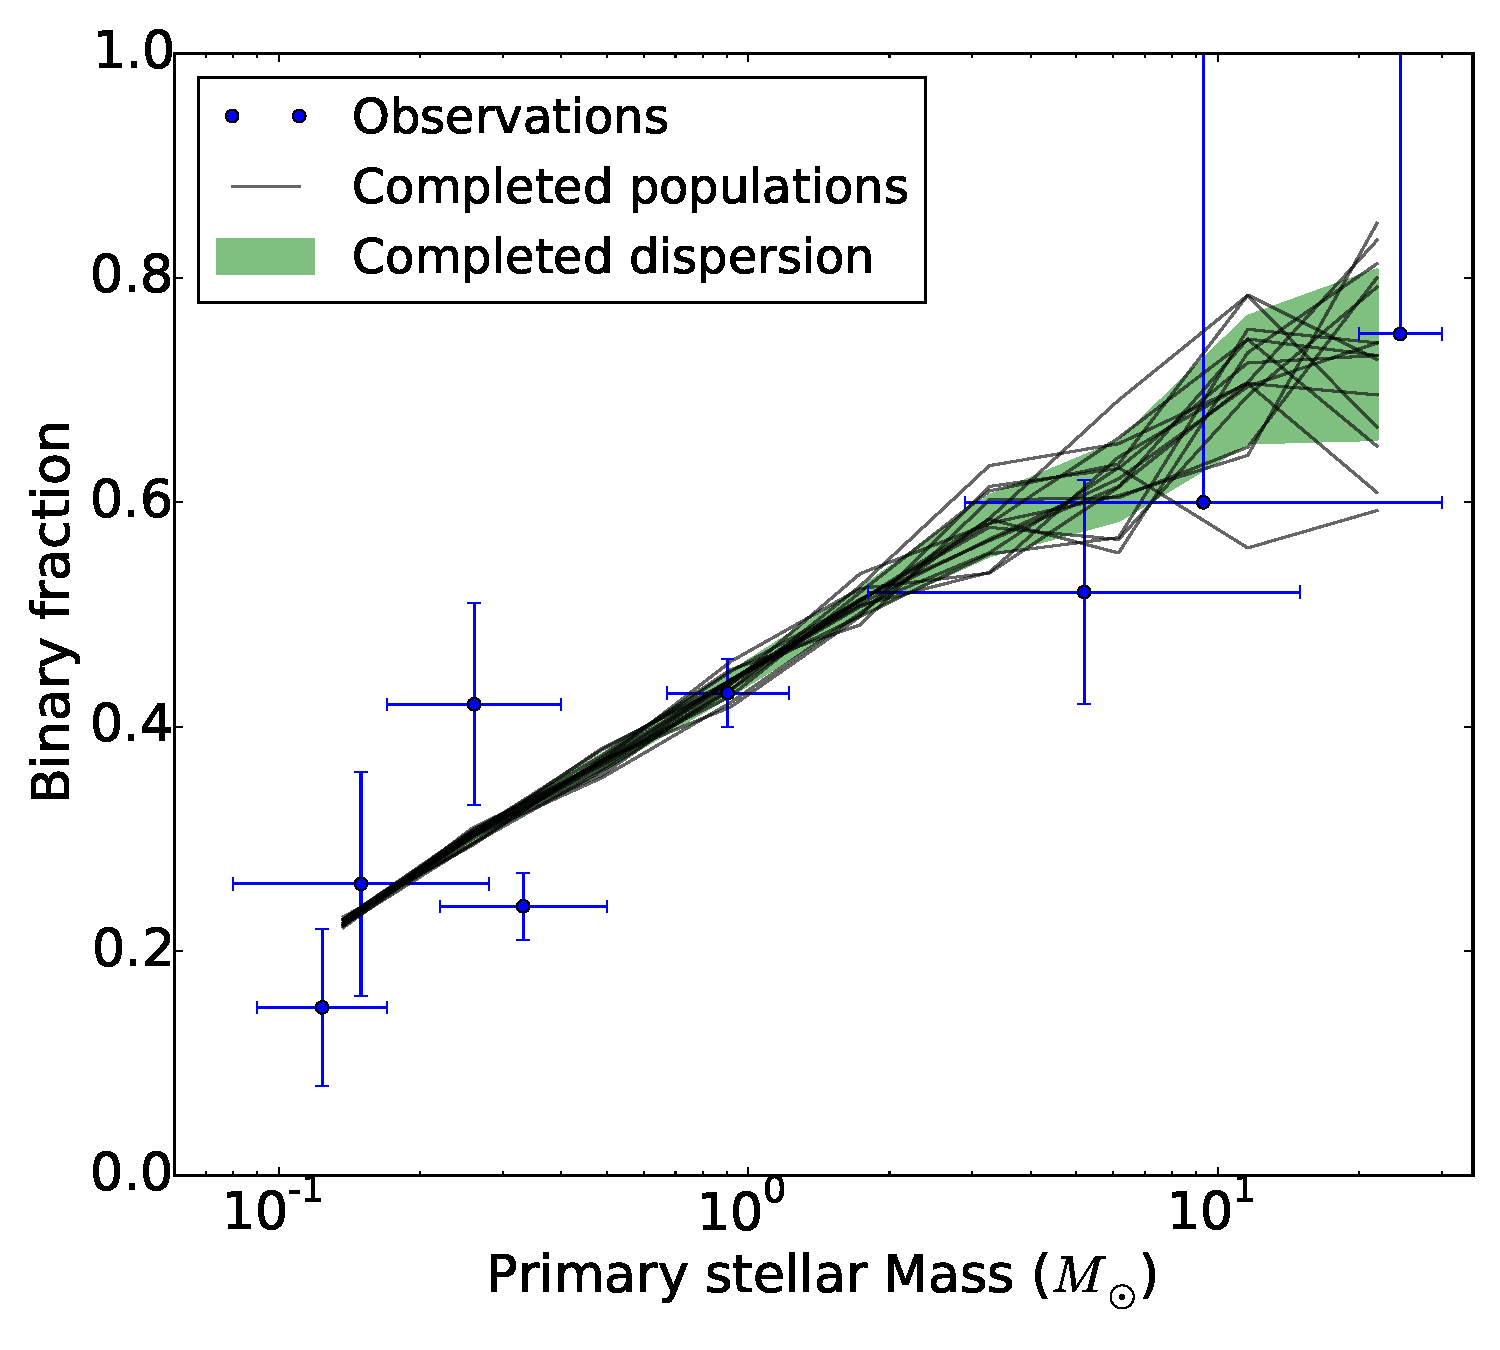
\includegraphics[width=0.7\textwidth]{Figures/5_completed_primarymass}
\caption{Binary fraction as a function of primary mass. The results displayed are the average of twenty realisations for 20k particles models; the shade indicates 1-$\sigma$ deviations. Short semi-major axis binaries were injected to complete the spontaneous population (compare with Fig~\protect\ref{Fig:5_spontaneous_primarymass}).}
\label{Fig:5_completed_primarymass}
\end{center}
\end{figure}

\subsubsection*{Result}

This procedure was tested on a new set of \HubLem twenty models, with the same parameters as before, N=20k, $L_3$ IMF, but with fused binaries injected in the system. The splitting was done twice for each model:  once with low density ($\approx 6$ stars$/\pc^3$), and once with high density ($\approx 400$ stars$/\pc^3$). The resulting binary fraction is plotted on Fig~\ref{Fig:5_completed_primarymass} as a function of the primary mass\footnote{Only the low mass primary models are shown, as density does not affect the primary-mass distribution.}. The deficit of low-mass primaries was bridged, while the fraction for high-mass primaries was slightly reduced (from 0.85 down to 0.75 for a primary mass of $\approx 20 \Mo$; note the increased scatter). This is the effect mentioned earlier, massive primaries see there secondary split into a system and the binary is destroyed. Enough high-mass binaries were injected so the fraction remains in complete agreement with observational data.

Turning to the distribution of semi-major axis, we choose to truncate the injected binary population at short semi-major axis. Extensive numerical exploration of binary tidal heating has been performed by O. Roos (2012, unpublished). Binaries were put on highly eccentric orbits in cuspy \cite{Dehnen1993} potentials, so experiencing large variations in the tidal force. It was found the binary's binding energy varied by $ \approx 50\%$ or more only when the semi-major axis $a >  100$ AU. No binary-single stars or binary-binary interactions were included. The conclusion from this study is that binaries with axis $a$ shorter than 100 AU should rarely unbind due to tidal heating. Further tests with NBODY6, and the results of the next section, largely confirm this. With that in mind, and in view of the computational costs, we truncated the binary population at $a = 1$ AU. This choice allows to recover the range found in the SPH calculations of \cite{Bate2012}, so a closer parallel can be made with his setup. 


We show on Fig~\ref{Fig:5_completed_smaxis} in short-dashed  the full spontaneous binary population (with a peak value at $a \approx 7 000$ AU), prior to the procedure to split fused binaries. The distribution of separations for the fused binaries is shown as the long-dashed blue curve, with a dip around $ a \approx 10 000$ and 2000 AU for low and high density. Finally, the splitting procedure is carried out, and the result shown as the solid green curve. The grey shade is the expectation value for
the parametrised Gaussian distribution of \cite{Raghavan2010}. Discrepancies with this distribution are only significant for binaries with $a > 4 000$ AU for both densities. For low-density models, the peak of the spontaneous population, still visible after the splitting procedure, introduces an excess of binaries for (roughly)  $ 4 000 < a < 20 000 $ AU. Note how the excess of binaries in that range has been halved by the splitting procedure, dropping from a maximum of $\approx 370$ to $ \approx 170$. For the high-density model, as the spontaneous population is shifted towards short separation, their inclusion is easier and they only introduce a slight bump in the distribution at $ a \sim 2 000 $ AU.

 For larger separations, the very wide binaries are not identified by the density threshold algorithm and are dropped from consideration. Since none of them are likely to survive for a long period of time given the density of the system, this will have no bearing on our conclusions. 

\paragraph*{}
While Hubble-Lemaitre fragmentation allows to obtain a self-consistent phase space distribution for a substructured model, the population completion presented here preserves this consistency by taking into account naturally occurring multiple systems, while allowing the user to inject a realistic binary population. 

In the next chapter, we use the resulting, completed systems as initial conditions to investigate the evolution of a binary population during the violent relaxation of a clumpy configuration.



\begin{figure}
    \centering
    \begin{subfigure}[b]{0.49\textwidth}
    	\centering
    	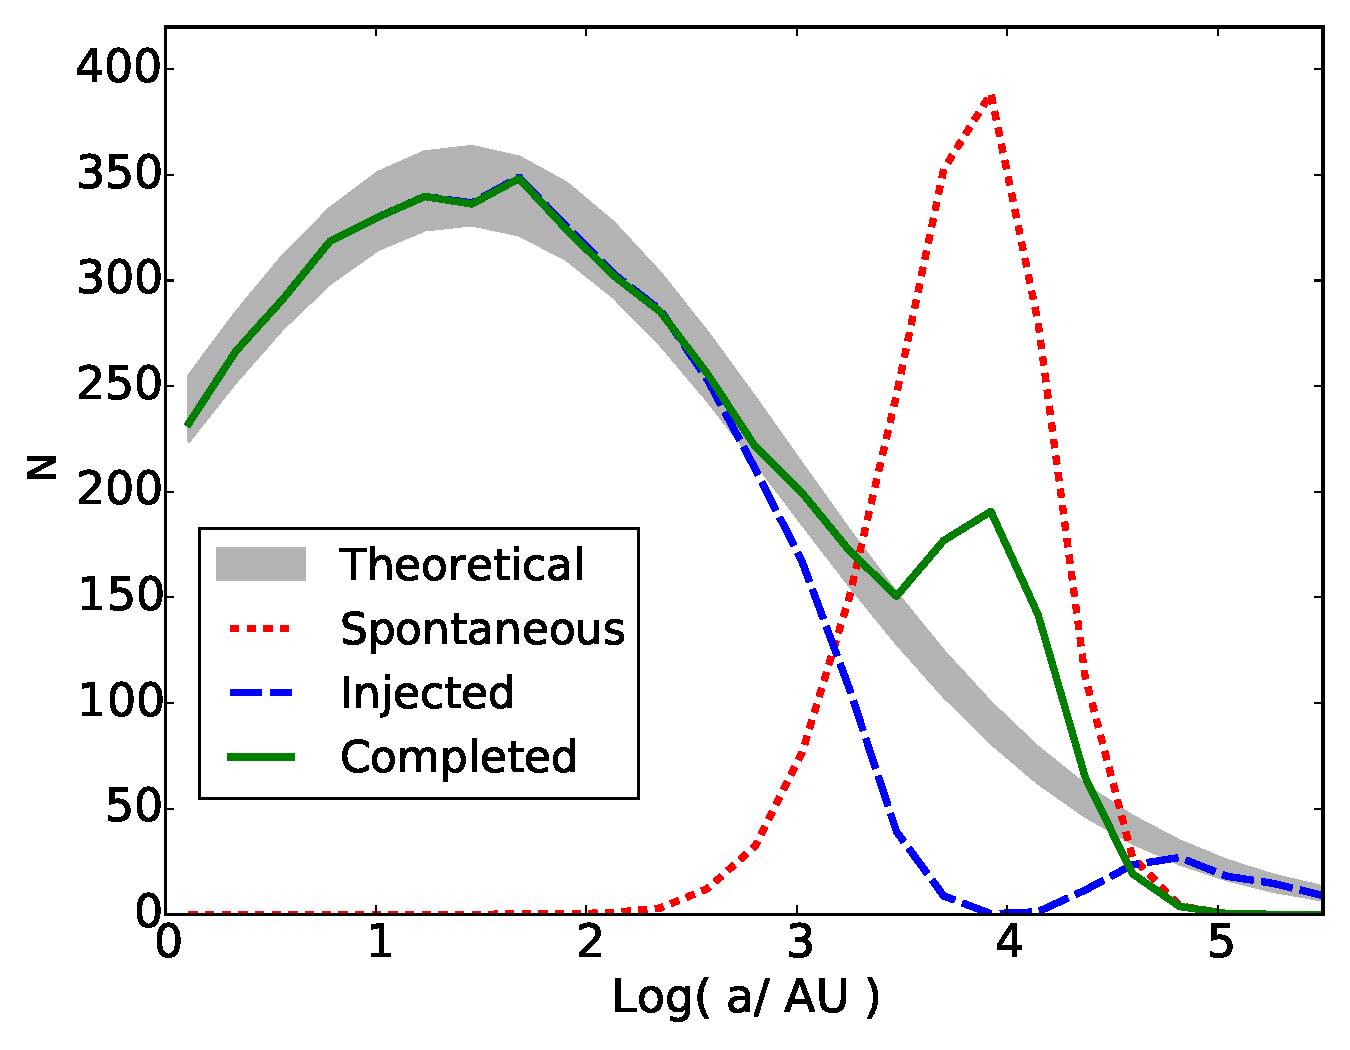
\includegraphics[width=\textwidth]{Figures/5_completed_smaxis_LD}
        \caption{Low-density model}
        \label{Fig:5_completed_smaxis_LD}
    \end{subfigure}
    \begin{subfigure}[b]{0.49\textwidth}
    	\centering
    	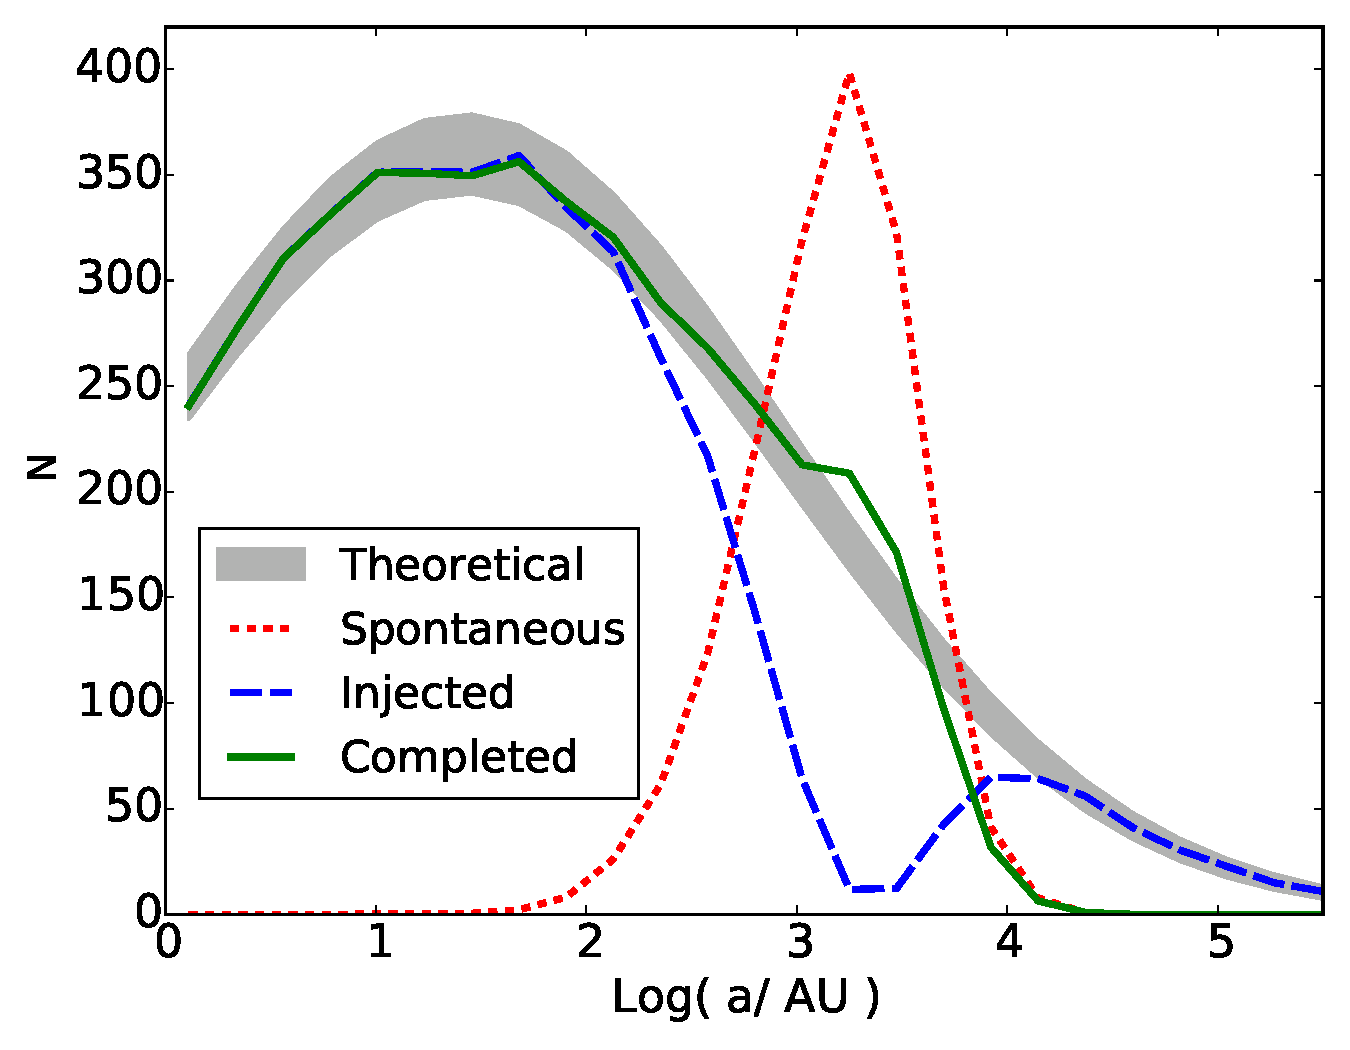
\includegraphics[width=\textwidth]{Figures/5_completed_smaxis_HD}
        \caption{High-density model}
        \label{Fig:5_completed_smaxis_HD}
    \end{subfigure}
\caption{Distributions of binary separations for the completion of a population in low and high density models. Spontaneous binaries before splitting are shown in short-dashed red, the population injected in the system in long-dashed blue and the resulting measured distribution in the completed system in green. The observational separation distribution from \protect\cite{Raghavan2010} is shown as a grey area, taking into account Poisson dispersion.}
\label{Fig:5_completed_smaxis}
\end{figure}

